% Created by tikzDevice version 0.12.6 on 2025-04-07 21:25:43
% !TEX encoding = UTF-8 Unicode
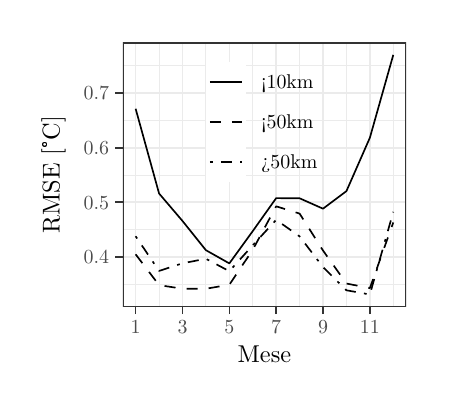
\begin{tikzpicture}[x=1pt,y=1pt]
\definecolor{fillColor}{RGB}{255,255,255}
\path[use as bounding box,fill=fillColor] (0,0) rectangle (142.26,128.04);
\begin{scope}
\path[clip] (  0.00,  0.00) rectangle (142.26,128.04);
\definecolor{drawColor}{RGB}{255,255,255}

\path[draw=drawColor,line width= 0.6pt,line join=round,line cap=round,fill=fillColor] (  0.00,  0.00) rectangle (142.26,128.04);
\end{scope}
\begin{scope}
\path[clip] ( 34.36, 27.29) rectangle (136.76,122.54);
\definecolor{fillColor}{RGB}{255,255,255}

\path[fill=fillColor] ( 34.36, 27.29) rectangle (136.76,122.54);
\definecolor{drawColor}{gray}{0.92}

\path[draw=drawColor,line width= 0.3pt,line join=round] ( 34.36, 35.38) --
	(136.76, 35.38);

\path[draw=drawColor,line width= 0.3pt,line join=round] ( 34.36, 55.10) --
	(136.76, 55.10);

\path[draw=drawColor,line width= 0.3pt,line join=round] ( 34.36, 74.82) --
	(136.76, 74.82);

\path[draw=drawColor,line width= 0.3pt,line join=round] ( 34.36, 94.53) --
	(136.76, 94.53);

\path[draw=drawColor,line width= 0.3pt,line join=round] ( 34.36,114.25) --
	(136.76,114.25);

\path[draw=drawColor,line width= 0.3pt,line join=round] ( 47.48, 27.29) --
	( 47.48,122.54);

\path[draw=drawColor,line width= 0.3pt,line join=round] ( 64.40, 27.29) --
	( 64.40,122.54);

\path[draw=drawColor,line width= 0.3pt,line join=round] ( 81.33, 27.29) --
	( 81.33,122.54);

\path[draw=drawColor,line width= 0.3pt,line join=round] ( 98.26, 27.29) --
	( 98.26,122.54);

\path[draw=drawColor,line width= 0.3pt,line join=round] (115.18, 27.29) --
	(115.18,122.54);

\path[draw=drawColor,line width= 0.3pt,line join=round] (132.11, 27.29) --
	(132.11,122.54);

\path[draw=drawColor,line width= 0.6pt,line join=round] ( 34.36, 45.24) --
	(136.76, 45.24);

\path[draw=drawColor,line width= 0.6pt,line join=round] ( 34.36, 64.96) --
	(136.76, 64.96);

\path[draw=drawColor,line width= 0.6pt,line join=round] ( 34.36, 84.67) --
	(136.76, 84.67);

\path[draw=drawColor,line width= 0.6pt,line join=round] ( 34.36,104.39) --
	(136.76,104.39);

\path[draw=drawColor,line width= 0.6pt,line join=round] ( 39.01, 27.29) --
	( 39.01,122.54);

\path[draw=drawColor,line width= 0.6pt,line join=round] ( 55.94, 27.29) --
	( 55.94,122.54);

\path[draw=drawColor,line width= 0.6pt,line join=round] ( 72.87, 27.29) --
	( 72.87,122.54);

\path[draw=drawColor,line width= 0.6pt,line join=round] ( 89.79, 27.29) --
	( 89.79,122.54);

\path[draw=drawColor,line width= 0.6pt,line join=round] (106.72, 27.29) --
	(106.72,122.54);

\path[draw=drawColor,line width= 0.6pt,line join=round] (123.65, 27.29) --
	(123.65,122.54);
\definecolor{drawColor}{RGB}{0,0,0}

\path[draw=drawColor,line width= 0.6pt,line join=round] ( 39.01, 98.75) --
	( 47.48, 68.12) --
	( 55.94, 58.20) --
	( 64.40, 47.64) --
	( 72.87, 42.86) --
	( 81.33, 54.53) --
	( 89.79, 66.44) --
	( 98.26, 66.39) --
	(106.72, 62.63) --
	(115.18, 68.97) --
	(123.65, 88.26) --
	(132.11,118.21);

\path[draw=drawColor,line width= 0.6pt,dash pattern=on 4pt off 4pt ,line join=round] ( 39.01, 46.14) --
	( 47.48, 35.01) --
	( 55.94, 33.71) --
	( 64.40, 33.70) --
	( 72.87, 35.15) --
	( 81.33, 47.77) --
	( 89.79, 63.49) --
	( 98.26, 60.86) --
	(106.72, 47.51) --
	(115.18, 35.59) --
	(123.65, 33.93) --
	(132.11, 57.65);

\path[draw=drawColor,line width= 0.6pt,dash pattern=on 1pt off 3pt on 4pt off 3pt ,line join=round] ( 39.01, 52.68) --
	( 47.48, 40.14) --
	( 55.94, 42.89) --
	( 64.40, 44.54) --
	( 72.87, 40.04) --
	( 81.33, 49.40) --
	( 89.79, 58.60) --
	( 98.26, 52.62) --
	(106.72, 41.52) --
	(115.18, 33.15) --
	(123.65, 31.62) --
	(132.11, 61.49);
\definecolor{drawColor}{gray}{0.20}

\path[draw=drawColor,line width= 0.6pt,line join=round,line cap=round] ( 34.36, 27.29) rectangle (136.76,122.54);
\end{scope}
\begin{scope}
\path[clip] (  0.00,  0.00) rectangle (142.26,128.04);
\definecolor{drawColor}{gray}{0.30}

\node[text=drawColor,anchor=base east,inner sep=0pt, outer sep=0pt, scale=  0.72] at ( 29.41, 42.78) {0.4};

\node[text=drawColor,anchor=base east,inner sep=0pt, outer sep=0pt, scale=  0.72] at ( 29.41, 62.49) {0.5};

\node[text=drawColor,anchor=base east,inner sep=0pt, outer sep=0pt, scale=  0.72] at ( 29.41, 82.21) {0.6};

\node[text=drawColor,anchor=base east,inner sep=0pt, outer sep=0pt, scale=  0.72] at ( 29.41,101.93) {0.7};
\end{scope}
\begin{scope}
\path[clip] (  0.00,  0.00) rectangle (142.26,128.04);
\definecolor{drawColor}{gray}{0.20}

\path[draw=drawColor,line width= 0.6pt,line join=round] ( 31.61, 45.24) --
	( 34.36, 45.24);

\path[draw=drawColor,line width= 0.6pt,line join=round] ( 31.61, 64.96) --
	( 34.36, 64.96);

\path[draw=drawColor,line width= 0.6pt,line join=round] ( 31.61, 84.67) --
	( 34.36, 84.67);

\path[draw=drawColor,line width= 0.6pt,line join=round] ( 31.61,104.39) --
	( 34.36,104.39);
\end{scope}
\begin{scope}
\path[clip] (  0.00,  0.00) rectangle (142.26,128.04);
\definecolor{drawColor}{gray}{0.20}

\path[draw=drawColor,line width= 0.6pt,line join=round] ( 39.01, 24.54) --
	( 39.01, 27.29);

\path[draw=drawColor,line width= 0.6pt,line join=round] ( 55.94, 24.54) --
	( 55.94, 27.29);

\path[draw=drawColor,line width= 0.6pt,line join=round] ( 72.87, 24.54) --
	( 72.87, 27.29);

\path[draw=drawColor,line width= 0.6pt,line join=round] ( 89.79, 24.54) --
	( 89.79, 27.29);

\path[draw=drawColor,line width= 0.6pt,line join=round] (106.72, 24.54) --
	(106.72, 27.29);

\path[draw=drawColor,line width= 0.6pt,line join=round] (123.65, 24.54) --
	(123.65, 27.29);
\end{scope}
\begin{scope}
\path[clip] (  0.00,  0.00) rectangle (142.26,128.04);
\definecolor{drawColor}{gray}{0.30}

\node[text=drawColor,anchor=base,inner sep=0pt, outer sep=0pt, scale=  0.72] at ( 39.01, 17.41) {1};

\node[text=drawColor,anchor=base,inner sep=0pt, outer sep=0pt, scale=  0.72] at ( 55.94, 17.41) {3};

\node[text=drawColor,anchor=base,inner sep=0pt, outer sep=0pt, scale=  0.72] at ( 72.87, 17.41) {5};

\node[text=drawColor,anchor=base,inner sep=0pt, outer sep=0pt, scale=  0.72] at ( 89.79, 17.41) {7};

\node[text=drawColor,anchor=base,inner sep=0pt, outer sep=0pt, scale=  0.72] at (106.72, 17.41) {9};

\node[text=drawColor,anchor=base,inner sep=0pt, outer sep=0pt, scale=  0.72] at (123.65, 17.41) {11};
\end{scope}
\begin{scope}
\path[clip] (  0.00,  0.00) rectangle (142.26,128.04);
\definecolor{drawColor}{RGB}{0,0,0}

\node[text=drawColor,anchor=base,inner sep=0pt, outer sep=0pt, scale=  0.88] at ( 85.56,  7.21) {Mese};
\end{scope}
\begin{scope}
\path[clip] (  0.00,  0.00) rectangle (142.26,128.04);
\definecolor{drawColor}{RGB}{0,0,0}

\node[text=drawColor,rotate= 90.00,anchor=base,inner sep=0pt, outer sep=0pt, scale=  0.88] at ( 11.56, 74.91) {RMSE [\textdegree C]};
\end{scope}
\begin{scope}
\path[clip] (  0.00,  0.00) rectangle (142.26,128.04);

\path[] ( 58.86, 66.78) rectangle (112.26,121.14);
\end{scope}
\begin{scope}
\path[clip] (  0.00,  0.00) rectangle (142.26,128.04);
\definecolor{fillColor}{RGB}{255,255,255}

\path[fill=fillColor] ( 64.36,101.19) rectangle ( 78.82,115.64);
\end{scope}
\begin{scope}
\path[clip] (  0.00,  0.00) rectangle (142.26,128.04);
\definecolor{drawColor}{RGB}{0,0,0}

\path[draw=drawColor,line width= 0.6pt,line join=round] ( 65.81,108.42) -- ( 77.37,108.42);
\end{scope}
\begin{scope}
\path[clip] (  0.00,  0.00) rectangle (142.26,128.04);
\definecolor{fillColor}{RGB}{255,255,255}

\path[fill=fillColor] ( 64.36, 86.74) rectangle ( 78.82,101.19);
\end{scope}
\begin{scope}
\path[clip] (  0.00,  0.00) rectangle (142.26,128.04);
\definecolor{drawColor}{RGB}{0,0,0}

\path[draw=drawColor,line width= 0.6pt,dash pattern=on 4pt off 4pt ,line join=round] ( 65.81, 93.96) -- ( 77.37, 93.96);
\end{scope}
\begin{scope}
\path[clip] (  0.00,  0.00) rectangle (142.26,128.04);
\definecolor{fillColor}{RGB}{255,255,255}

\path[fill=fillColor] ( 64.36, 72.28) rectangle ( 78.82, 86.74);
\end{scope}
\begin{scope}
\path[clip] (  0.00,  0.00) rectangle (142.26,128.04);
\definecolor{drawColor}{RGB}{0,0,0}

\path[draw=drawColor,line width= 0.6pt,dash pattern=on 1pt off 3pt on 4pt off 3pt ,line join=round] ( 65.81, 79.51) -- ( 77.37, 79.51);
\end{scope}
\begin{scope}
\path[clip] (  0.00,  0.00) rectangle (142.26,128.04);
\definecolor{drawColor}{RGB}{0,0,0}

\node[text=drawColor,anchor=base west,inner sep=0pt, outer sep=0pt, scale=  0.72] at ( 84.32,105.95) {<10km};
\end{scope}
\begin{scope}
\path[clip] (  0.00,  0.00) rectangle (142.26,128.04);
\definecolor{drawColor}{RGB}{0,0,0}

\node[text=drawColor,anchor=base west,inner sep=0pt, outer sep=0pt, scale=  0.72] at ( 84.32, 91.50) {<50km};
\end{scope}
\begin{scope}
\path[clip] (  0.00,  0.00) rectangle (142.26,128.04);
\definecolor{drawColor}{RGB}{0,0,0}

\node[text=drawColor,anchor=base west,inner sep=0pt, outer sep=0pt, scale=  0.72] at ( 84.32, 77.05) {>50km};
\end{scope}
\end{tikzpicture}
